

\begin{section}{Condiciones de contorno}
El sistema físico esta compuesto por un recipiente rectangular que contiene un liquido dentro. Ademas una hélice en el centro, cuyas aspas son rectas y de exactamente la misma longitud a distintas alturas, perturba el liquido produciendo en el cambios de velocidad. 
Para la simulación se aprovechara la simetría del problema para modelarlo en dos dimensiones. Se tomara entonces un corte horizontal del reactor. El sistema, como sera modelado, consiste entonces de un plano horizontal, cuyos vértices y aristas representan las paredes del recipiente, un espacio dentro que representa el fluido, y segmentos en el centro que representan la posición de las aspas de la hélice. Definir la cantidad de aspas en la hélice es sencillo, basta con cambiar las condiciones en un condicional que logra que se trate distinto a los elementos de fluido donde debería estar un aspa. En el presente trabajo se realizó la experimentación con una única aspa ya que esto aporta mayor claridad a la hora de evaluar el comportamiento del fluido.
~\\


\begin{figure}[h]
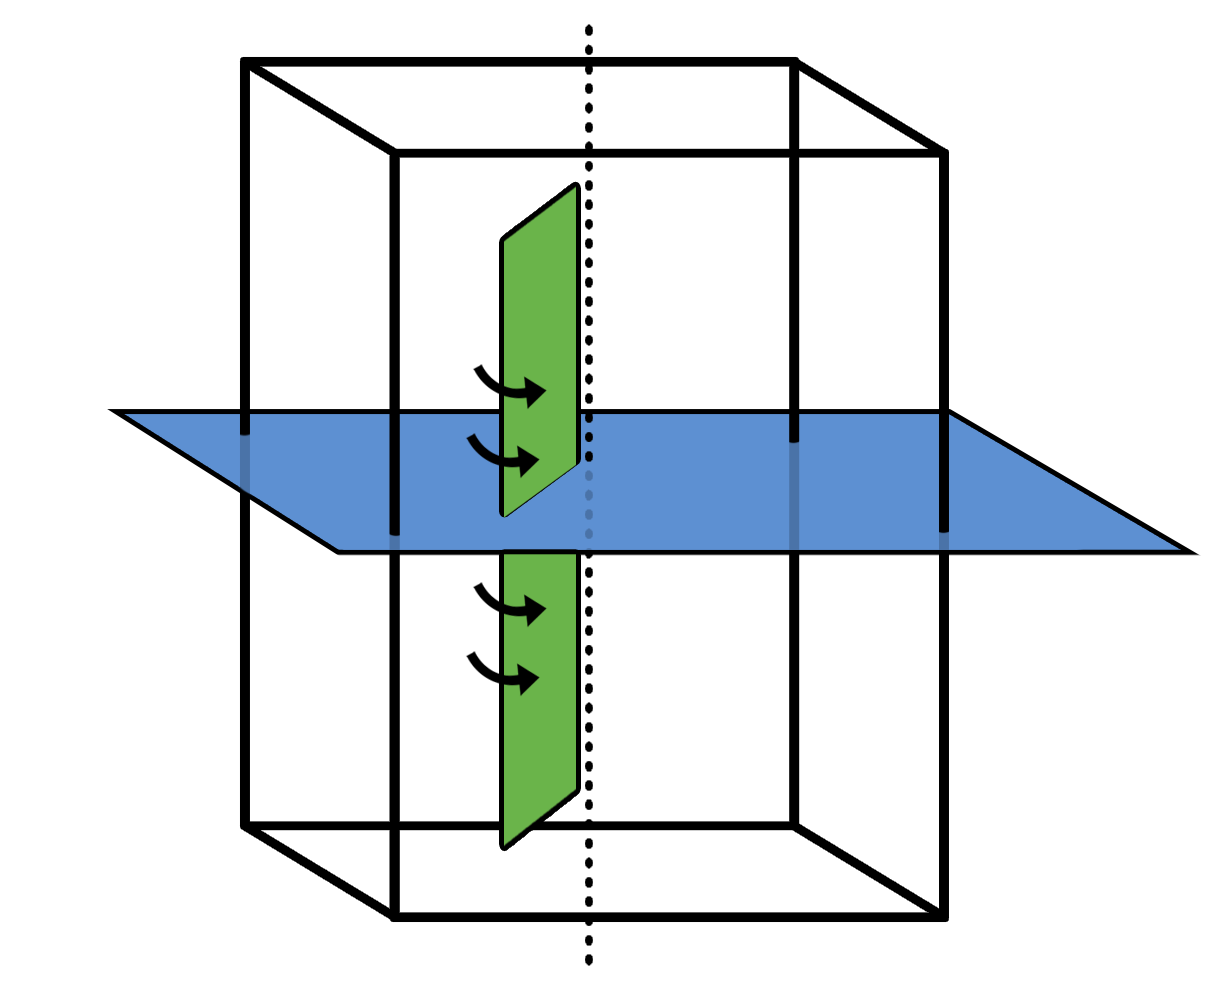
\includegraphics[width=\textwidth/2,height=\textheight/2,keepaspectratio]{figures/reactor}
\caption{Esquema del sistema físico modelado.}
\label{fig:border}

\end{figure}

~\\
Las condiciones de contorno para Las ecuaciones de velocidad no presentan mayores complejidades, se establece la velocidad del fluido en los bordes del contenedor como cero en ambas direcciones, u y v. Estas velocidades no se cambian en las subsecuentes iteraciones del programa ya que representan las paredes del contenedor que se mantienen quietas en todo momento en el sistema físico real.
En cuanto a la ecuación de la presión, utilizar una presión de cero en el contorno no seria realista dado que la presencia de una  presión muy baja produce la atracción del fluido circundante. Una forma de deducir el valor correcto de la presión en los bordes del contenedor es utilizar las ecuaciones de Newton. Si un elemento de fluido realiza una fuerza en la pared del contenedor, dado que esta no se mueve, devuelve una fuerza igual al elemento de fluido. Realizando este calculo, se llega a una condición de igualdad entre el elemento de borde y el elemento de fluido que se encuentre junto a este. Básicamente lo que ese resultado nos dice es que el valor de presión para un elemento de borde debe ser el mismo que el del elemento de fluido que esta junto a el, pudiendo entonces solucionar este aspecto de la simulación simplemente copiando el valor del elemento de fluido mas cercano a cada elemento de borde en cada iteración.\\
Finalmente para las condiciones iniciales, se estableció la velocidad en u y en v en cero para todo el sistema.

\end{section}
